\subsection{Demonstration}
\begin{frame}
    
\begin{center}
    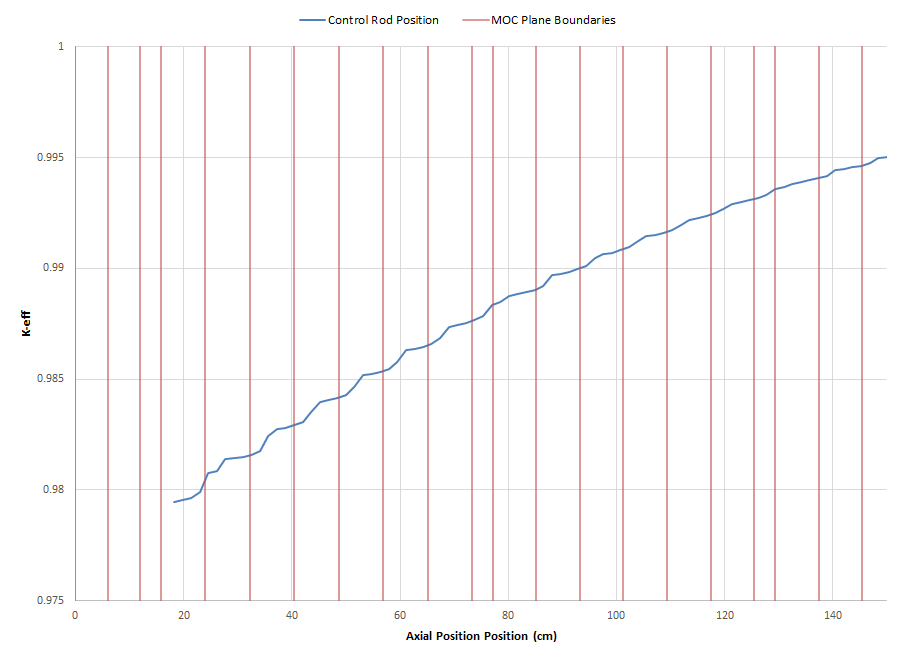
\includegraphics[width=0.8\textwidth]{p4cuspingEffects.png}
\end{center}
\vfill
    
\end{frame}

%%%%%%%%%%%%%%%%%%%%%%%%%%%%%%%%%%%%%%%%%%%%%%%%%%%%%%%%%%%%%%%%%%%%%%%%%%%%%%%%%

\subsection{Previous Decusping Methods}
\begin{frame}[t]{2D/1D Decusping Methods}

\begin{itemize}
\item Neighbor Spectral Index Method - CRX-2K 
\cite{cho2015CRX2d1dFusionDecusping}
\begin{itemize}
    \item Spectral index is defined as the ratio of the fast flux to the 
    thermal flux
    \item Spectral index is used in top and bottom neighbor nodes to 
    estimate partially rodded node flux profile
    \item This estimate is used to update cross sections 
    each iteration
\end{itemize}
\item nTRACER Method \cite{ICAPPcontrolRodDecuspingNTRACER}
\begin{itemize}
    \item Solves local problem to generate CMFD constants
    \item Performs CMFD calculations on fine mesh to obtain axial flux 
    profiles
    \item Uses axial flux profiles during full core calculation to 
    homogenize cross sections
\end{itemize}
\item Approximate Flux Weighting Method \cite{gehinThesis1992quasi}
\begin{itemize}
    \item Originally developed for nodal methods, but also implemented in nTRACER \cite{Ryu2017nTRACERWholeCoreTransportSolutionstoC5G7-TDBenchmark}
    \item Assumes that in partially rodded node, rodded flux is similar to node above and unrodded flux is similar to node below
    \item Assumption allows the partially rodded node cross section to be updated easily during iteration
\end{itemize}
\end{itemize}

\end{frame}

%%%%%%%%%%%%%%%%%%%%%%%%%%%%%%%%%%%%%%%%%%%%%%%%%%%%%%%%%%%%%%%%%%%%%%%%%%%%%%%%%

\begin{frame}[t]{Methods Shortcomings}
    
    \begin{itemize}
        \item Extensive research has been done on decusping methods, primarily for nodal codes
        \item Several methods have been developed for 2D/1D codes
        \begin{itemize}
            \item Some methods involved coarse approximations with limited accuracy
            \item Others required expensive additional calculations that increased runtime of the code significantly
        \end{itemize}
        \item New methods need to improve on prior ones by providing more accurate solutions without significantly slowing down calculations
    \end{itemize}

\end{frame}